\chapter{Esercitazioni su IPv4: Indirizzamento, Routing e Cattura Pacchetti}

In questo capitolo vengono affrontati una serie di esercizi pratici riguardanti l'indirizzamento IPv4, la definizione di Netmask e prefissi di rete, il subnetting, l'aggregazione nelle tabelle di routing e l'analisi del traffico di rete (tramite cattura pacchetti). 

Una precisazione preliminare sulla notazione utilizzata in queste esercitazioni e nelle tabelle di routing: per le \textbf{rotte direttamente connesse} verrà utilizzata la lettera \textbf{C} (Connected), e verrà assegnato loro un \textbf{costo pari a 0}. Questa notazione rispecchia lo standard maggiormente diffuso nella pratica (ad esempio nei dispositivi Cisco). Le rotte statiche inserite manualmente dall'amministratore saranno indicate con la lettera \textbf{S}.

\section{Calcolo di Netmask e Prefissi di Rete}

Il primo problema pratico nella progettazione di una rete consiste nel determinare il prefisso di rete (Prefix Length) e la relativa Netmask necessari per ospitare un determinato numero di host. 

Per risolvere questo problema si può ricorrere alla rappresentazione binaria degli indirizzi, ma un metodo spesso più rapido consiste nel ragionare in \textbf{decimale}, utilizzando le potenze del 2. 

\subsection{Metodo basato sulle potenze del 2}
Se si necessita di un certo numero di host, si deve trovare la potenza del 2 immediatamente superiore che possa contenerli, ricordando sempre che \textbf{due indirizzi sono riservati} (uno per identificare la rete stessa, ovvero il Network ID, e uno per il Broadcast). Il calcolo del numero di indirizzi utili è sempre:
\[ \text{Indirizzi disponibili} = 2^n - 2 \]
dove \( n \) è il numero di bit dedicati alla parte host.

Per calcolare rapidamente il valore decimale da inserire nel byte interessato della Netmask (che non è 255), invece di sottrarre il valore binario massimo rappresentabile (es. $255 - 3$), si consiglia di utilizzare la seguente formula:
\[ \text{Valore Byte Netmask} = 256 - 2^n \]
dove \( 256 \) è pari a $2^8$ (il numero totale di combinazioni su 8 bit) e \( 2^n \) è il numero totale di indirizzi IP (inclusi rete e broadcast) forniti dai bit di host presenti \textit{in quel byte}.

\begin{example}[Calcolo per 2 host]
Vogliamo una subnet per collegare 2 host (tipico dei collegamenti punto-punto). Ci servono in totale 4 indirizzi IP ($2 + 2$ riservati). 
Poiché $4 = 2^2$, ci servono 2 bit per gli host. Il prefisso di rete sarà quindi $32 - 2 = \textbf{/30}$.
Applicando la formula per il quarto byte: $256 - 2^2 = 256 - 4 = 252$.
La Netmask sarà: \texttt{255.255.255.252}.
\end{example}

\begin{example}[Calcolo per 27 host]
Servono almeno $27 + 2 = 29$ indirizzi. La potenza del due utile è 32 ($2^5$). 
Ci servono 5 bit per l'host. Prefisso: $32 - 5 = \textbf{/27}$.
Valore del quarto byte: $256 - 2^5 = 256 - 32 = 224$.
La Netmask sarà: \texttt{255.255.255.224}.
\end{example}

\begin{example}[Calcolo per 300 host (cambio di byte)]
Servono almeno 302 indirizzi. La potenza del due sufficiente è 512 ($2^9$).
Ci servono 9 bit per gli host. Questo significa che il prefisso di rete sarà $32 - 9 = \textbf{/23}$.
Poiché i bit di host invadono il terzo byte (1 bit nel terzo byte e 8 bit nel quarto), il quarto byte della Netmask sarà a 0.
Per il terzo byte applichiamo la formula considerando solo il bit di host che "sborda" in questo byte ($n=1$):
\[ \text{Valore 3° Byte} = 256 - 2^1 = 256 - 2 = 254 \]
La Netmask sarà: \texttt{255.255.254.0}.
\end{example}

\subsection{Tabella riassuntiva di calcolo}

La seguente tabella riassume i calcoli per diverse richieste di host, mostrando come si ricavano la Netmask, la Prefix Length e gli indirizzi disponibili.

\begin{table}[H]
    \centering
    \begin{tabular}{|c|c|c|c|}
        \hline
        \textbf{Numero di Host} & \textbf{Netmask} & \textbf{Prefix Length} & \textbf{Indirizzi Disponibili} \\
        \hline
        2 & 255.255.255.252 & /30 & 4 (-2) \\
        \hline
        27 & 255.255.255.224 & /27 & 32 (-2) \\
        \hline
        5 & 255.255.255.248 & /29 & 8 (-2) \\
        \hline
        100 & 255.255.255.128 & /25 & 128 (-2) \\
        \hline
        10 & 255.255.255.240 & /28 & 16 (-2) \\
        \hline
        300 & 255.255.254.0 & /23 & 512 (-2) \\
        \hline
        1010 & 255.255.252.0 & /22 & 1024 (-2) \\
        \hline
        55 & 255.255.255.192 & /26 & 64 (-2) \\
        \hline
        167 & 255.255.255.0 & /24 & 256 (-2) \\
        \hline
        1540 & 255.255.248.0 & /21 & 2048 (-2) \\
        \hline
    \end{tabular}
    \caption{Risoluzione del dimensionamento delle subnet.}
    \label{tab:subnet_sizing}
\end{table}

\section{Verifica della Validità di un Prefisso di Rete}

Un indirizzo IP associato a una prefix length (es. \texttt{192.168.2.36/29}) rappresenta un \textbf{prefisso di rete valido} solo se \textbf{tutti i bit della parte host sono posti a zero}. Se vi sono dei bit a uno nella parte host, l'indirizzo rappresenta un host specifico all'interno di una rete, e non l'identificativo della rete stessa.

Anche in questo caso, è possibile verificare la validità ragionando sui multipli decimali anziché convertire in binario:
\begin{itemize}
    \item Se la rete ha $n$ bit di host nel byte analizzato, l'identificativo di rete valido (che ha tutti quegli $n$ bit a 0) deve essere \textbf{un multiplo di \( 2^n \)}.
\end{itemize}

\begin{example}[Analisi di 192.168.2.36/29 e /30]
Consideriamo l'indirizzo \texttt{192.168.2.36}.
\begin{itemize}
    \item È valido per un \textbf{/30}? Un /30 ha 2 bit di host ($2^2=4$). Il numero 36 è un multiplo di 4? Sì ($36 = 9 \times 4$). Quindi \texttt{192.168.2.36/30} è una rete valida.
    \item È valido per un \textbf{/29}? Un /29 ha 3 bit di host ($2^3=8$). Il numero 36 è un multiplo di 8? No (i multipli sono 32, 40). Quindi \texttt{192.168.2.36/29} \textbf{non} è valido. La rete corretta a cui appartiene l'host .36 è \texttt{192.168.2.32/29} (che si estende fino a .39).
\end{itemize}
\end{example}

\begin{remark}[Il caso del /31]
Il prefisso \textbf{/31} (come \texttt{192.168.2.0/31}) genera reti di $2^1 = 2$ indirizzi. Tuttavia, dovendo sottrarre rete e broadcast ($2-2=0$), non rimarrebbero indirizzi utili per gli host. Pertanto, nel subnetting tradizionale, il /31 \textbf{non è considerato valido}; la subnet più piccola utilizzabile è la /30.
\end{remark}

\begin{table}[H]
    \centering
    \begin{tabular}{|l|c|}
        \hline
        \textbf{Coppia IP / Prefix Length} & \textbf{Rete Valida?} \\
        \hline
        192.168.5.0/24 & SÌ \\
        \hline
        192.168.4.23/24 & NO (23 non è multiplo di 256, l'host parte da 0) \\
        \hline
        192.168.2.36/30 & SÌ \\
        \hline
        192.168.2.36/29 & NO (36 non è multiplo di 8, la rete è .32) \\
        \hline
        192.168.2.32/28 & SÌ (32 è multiplo di 16) \\
        \hline
        192.168.2.32/27 & SÌ (32 è multiplo di 32) \\
        \hline
        192.168.3.0/23 & NO (Nel terzo byte, 3 è dispari. I multipli di $2^1=2$ sono pari) \\
        \hline
        192.168.2.0/31 & NO!!! (Non rimangono indirizzi per gli host) \\
        \hline
        192.168.2.0/23 & SÌ (Nel terzo byte, 2 è multiplo di 2) \\
        \hline
        192.168.16.0/21 & SÌ (Nel terzo byte, 16 è multiplo di $2^3=8$) \\
        \hline
        192.168.12.0/21 & NO (12 non è multiplo di 8) \\
        \hline
    \end{tabular}
    \caption{Verifica della validità dei prefissi di rete.}
    \label{tab:valid_prefixes}
\end{table}


\section{Analisi degli Errori di Configurazione}

Si consideri il seguente scenario di rete, al fine di individuare l'errore di configurazione:
\begin{itemize}
    \item \textbf{Router:} IP 192.168.0.1/24 (su interfaccia sinistra), IP 192.168.1.1/28 (su interfaccia destra)
    \item \textbf{DNS 1:} IP 192.168.0.23/24, DG: 192.168.0.1, DNS: 192.168.0.23
    \item \textbf{Host 1:} IP 192.168.0.2/24, DG: 192.168.0.1, DNS: 192.168.1.23
    \item \textbf{DNS 2:} IP 192.168.1.23/28, DG: 192.168.1.1, DNS: 192.168.1.23

    \begin{figure}[H]
        \centering
        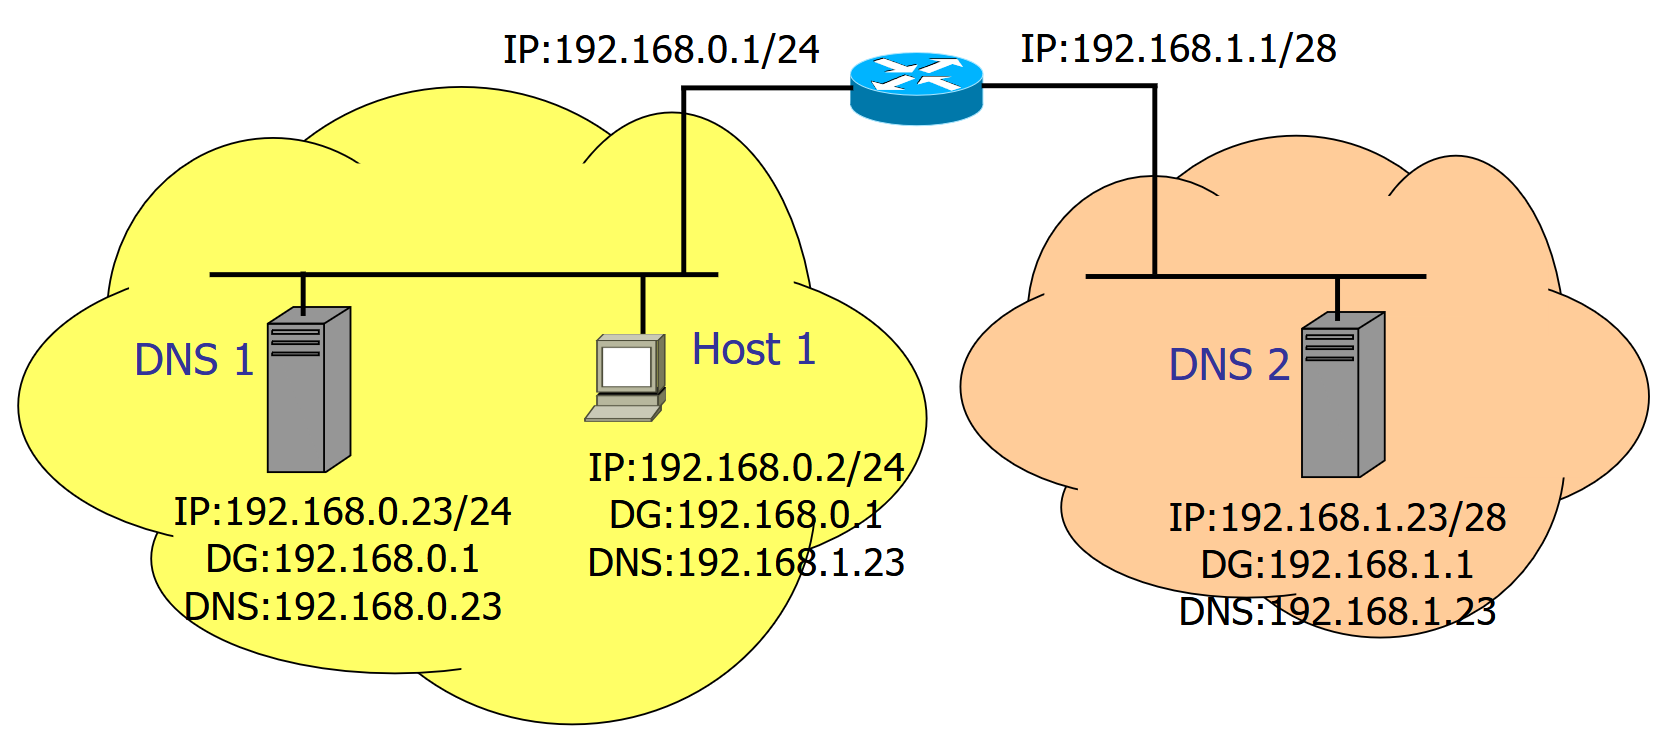
\includegraphics[width=0.7\textwidth]{capitoli/01b - IPv4 ExerciseSummary/images/placeholder_config_error}
        \caption{Topologia di rete per l'analisi dell'errore di configurazione.}
    \end{figure}

\end{itemize}

\textbf{Diagnosi dell'errore:}
L'errore risiede nella configurazione della porzione di rete destra, che include l'interfaccia del Router (\texttt{192.168.1.1/28}) e il DNS 2 (\texttt{192.168.1.23/28}). 
Un prefisso \textbf{/28} fornisce blocchi di 16 indirizzi ($2^4$). 
La rete del Router parte da \texttt{192.168.1.0/28} e si estende fino all'host utile \texttt{192.168.1.14} (con \texttt{.15} come broadcast). 
L'indirizzo del DNS 2 (\texttt{192.168.1.23}) appartiene alla subnet successiva, ovvero \texttt{192.168.1.16/28} (che termina a \texttt{.31}). 
Di conseguenza, Router e DNS 2 credono di essere nella stessa rete fisica, ma a livello logico (IP) non si trovano nella stessa subnet. Il DNS 2 non può quindi comunicare con l'esterno, poiché non riuscirà a contattare il Default Gateway.

\textbf{Osservazione:} Il fatto che Host 1 (che si trova a sinistra) utilizzi il DNS 2 (che si trova a destra, con IP \texttt{192.168.1.23}) \textbf{non è un errore}. L'utilizzo di un server DNS remoto (esterno alla propria subnet) è una pratica perfettamente normale e valida, purché il server sia raggiungibile tramite routing (cosa che qui fallisce per l'errore precedente).


\section{Pianificazione dell'Indirizzamento IP (Subnetting)}

Quando viene fornito uno spazio di indirizzamento (address range) per un'azienda, ad esempio \texttt{10.0.0.0/24}, è necessario allocare i prefissi di rete alle diverse LAN in modo coerente.

% FIGURA ORIGINALE DA RECUPERARE DALLE SLIDE
% Slide di provenienza: 9
% Tipo: diagramma
% Descrizione: Topologia di rete con un router centrale connesso a LAN1 (350 host), LAN2 (120 host) e un collegamento punto-punto. (L'indirizzo di partenza è indicato come 10.0.0.0/16, ma si decide di operare con un range più piccolo)
% Punto di inserimento: Inizio spiegazione pianificazione indirizzamento
% File da inserire: topologia_lan1_lan2_link

\begin{figure}[H]
    \centering
    % Sostituire il segnaposto con il percorso effettivo dell'immagine
    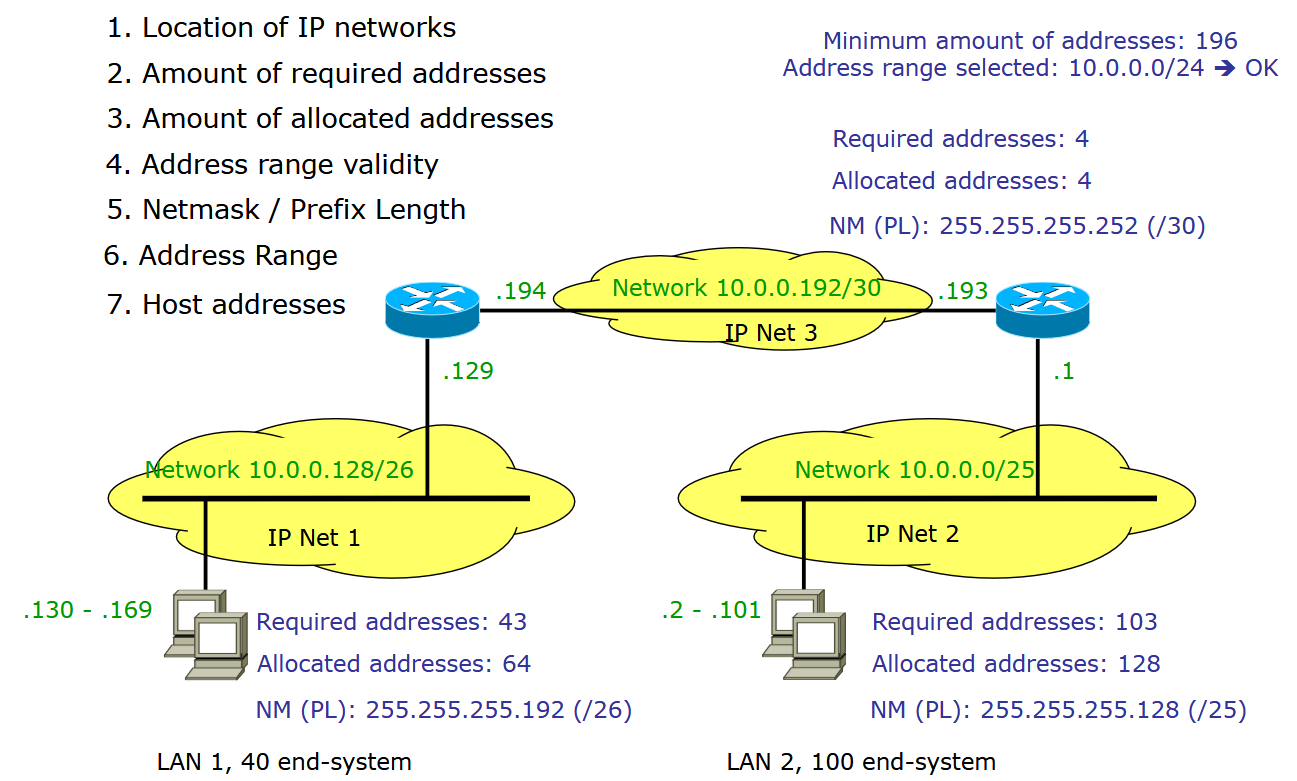
\includegraphics[width=0.85\textwidth]{capitoli/01b - IPv4 ExerciseSummary/images/topologia_lan1_lan2_link}
    \caption{Topologia per l'esercizio di pianificazione dell'indirizzamento.}
    \label{fig:addressing_topo}
\end{figure}

\subsection{Regole e calcolo dei requisiti}
La prima operazione da compiere è determinare il fabbisogno effettivo di indirizzi IP per ogni dominio di collisione/broadcast (LAN). 
Una svista comune è considerare solo il numero di host dichiarati. Il numero minimo di indirizzi IP richiesti in una subnet è dato da:
\[ \text{IP Req} = \text{Numero Host} + 3 \]
I 3 indirizzi extra derivano da:
\begin{enumerate}
    \item \textbf{Indirizzo di Rete} (Network ID, tutti 0 nella parte host).
    \item \textbf{Indirizzo di Broadcast} (tutti 1 nella parte host).
    \item \textbf{Interfaccia del Router} (anche il router è un dispositivo della LAN e necessita di un indirizzo IP in quella subnet, spesso il primo o l'ultimo disponibile).
\end{enumerate}

Nell'esempio della figura (se avessimo un range \texttt{/24}):
\begin{itemize}
    \item \textbf{LAN Link punto-punto:} 2 host (interfacce router) $\rightarrow$ Servono 4 indirizzi. Si alloca una \textbf{/30} (alloca 4 IP).
    \item \textbf{LAN 1:} 40 host dichiarati $\rightarrow$ Ne servono almeno 43. Potenza del due successiva: 64 ($2^6$). Si alloca una \textbf{/26}.
    \item \textbf{LAN 2:} 100 host dichiarati $\rightarrow$ Ne servono almeno 103. Potenza del due successiva: 128 ($2^7$). Si alloca una \textbf{/25}.
    \item (Attenzione: se si avessero 126 host dichiarati, servirebbero $126+3=129$ indirizzi, rendendo necessaria una /24 da 256 indirizzi. Centoventisei è il caso limite su cui bisogna prestare attenzione).
\end{itemize}

Un controllo fondamentale da fare a monte è verificare se lo spazio address range assegnato sia sufficiente. \textbf{Si devono sommare gli indirizzi allocati (le potenze di 2 scelte), NON quelli strettamente richiesti.}
Esempio: In un \texttt{/24} abbiamo 256 IP. Allocando una /25 (128 IP), una /26 (64 IP) e una /30 (4 IP), la somma è $128 + 64 + 4 = 196$. Poiché $196 \le 256$, lo spazio è sufficiente.

\subsection{Approcci all'allocazione}
Una volta determinati i prefissi necessari, come li posizioniamo all'interno dell'address range \texttt{10.0.0.0/24}?

\textbf{1. Approccio "Tradizionale" (Sequenziale)}
Si assegna partendo dalla LAN 1, poi la LAN 3 (link), poi la LAN 2. Questo approccio procede per tentativi e può generare blocchi in quanto alcuni indirizzi (come i limiti delle subnet) non risultano multipli corretti delle potenze di 2, rendendoli "invalidi" per la Prefix Length desiderata. Crea spesso frammentazione.

\textbf{2. Soluzione Best Practice (Dalla più grande alla più piccola)}
Il metodo più pulito per evitare problemi di allineamento e sprechi frammentati è \textbf{allocare le subnet partendo da quella che richiede più indirizzi e procedendo in ordine decrescente}.
\begin{itemize}
    \item \textbf{LAN 2 (128 IP, /25):} Parte da \texttt{10.0.0.0/25}. Termina a \texttt{.127}.
    \item \textbf{LAN 1 (64 IP, /26):} Parte da \texttt{10.0.0.128/26}. Questo è valido perché 128 è multiplo di 64. Termina a \texttt{.191}.
    \item \textbf{LAN Link (4 IP, /30):} Parte da \texttt{10.0.0.192/30}. Valido in quanto 192 è multiplo di 4. Termina a \texttt{.195}.
\end{itemize}
Tutti gli indirizzi IP liberi rimangono alla fine del range (da \texttt{.196} a \texttt{.255}), garantendo flessibilità per espansioni future.

\textbf{3. Soluzione Minimizzazione degli IP sprecati}
Se ci trovassimo in un caso dove per 350 host allocassimo una /23 (512 IP), sprecheremmo molti indirizzi. Se si vuole ottimizzare rigorosamente lo spreco, è possibile definire \textbf{più subnet logiche sulla stessa LAN fisica}.
Invece di usare una /23 per 350 host, si possono definire sulla stessa rete fisica una \texttt{/24} (256 IP) e una \texttt{/25} (128 IP). $256 + 128 = 384 > 350$.
Questo approccio riduce enormemente lo spreco, ma ha due conseguenze:
\begin{enumerate}
    \item Gli host fisicamente nella stessa stanza si troveranno su subnet logiche differenti.
    \item Il router dovrà possedere \textbf{due indirizzi IP} configurati sulla medesima interfaccia fisica (uno per la subnet /24 e uno per la /25).
\end{enumerate}
Benché tecnicamente ineccepibile, la complessità di gestione (frammentazione) rende la Soluzione 2 il compromesso "trade-off" preferito nel 99\% degli scenari pratici, lasciando spazio all'elasticità per modifiche future senza dover riprogettare l'intera configurazione.


\section{Tabelle di Routing e Aggregazione delle Rotte}

L'assegnazione degli indirizzi IP non è fine a se stessa, ma impatta pesantemente sulla \textbf{tabella di routing} dei dispositivi core. Una corretta allocazione permette l'\textbf{aggregazione} delle rotte (Route Summarization), riducendo le dimensioni della routing table.

% FIGURA ORIGINALE DA RECUPERARE DALLE SLIDE
% Slide di provenienza: 12
% Tipo: diagramma
% Descrizione: Topologia per tabella di routing R2, con R1 a sinistra e R3 (internet) a destra. Mostra LAN 130.192.2.0/26 e 130.192.2.128/25.
% Punto di inserimento: Qui, per far comprendere la tabella sottostante.
% File da inserire: topologia_routing_R2

\begin{figure}[H]
    \centering
    % Sostituire il segnaposto con il percorso effettivo dell'immagine
    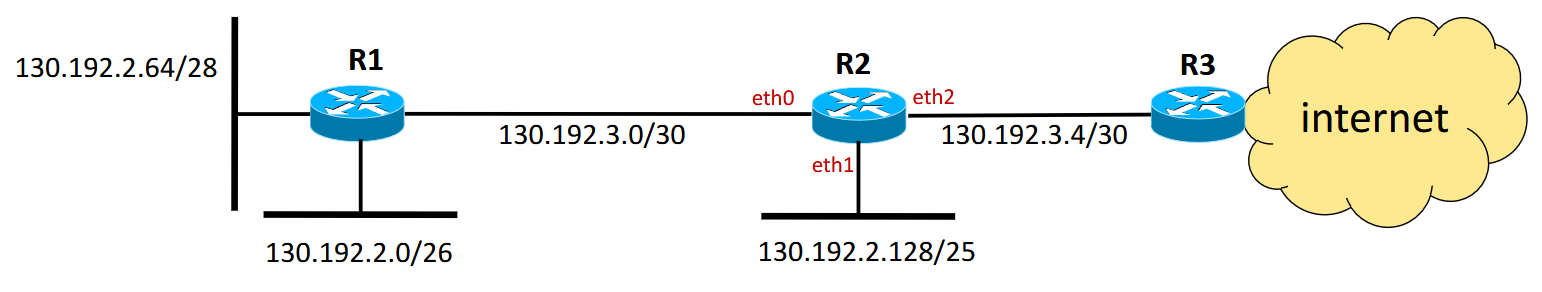
\includegraphics[width=0.85\textwidth]{capitoli/01b - IPv4 ExerciseSummary/images/topologia_routing_R2}
    \caption{Rete per la determinazione della tabella di routing di R2.}
    \label{fig:routing_r2}
\end{figure}

Nella costruzione delle tabelle:
\begin{itemize}
    \item Le rotte connesse (\textbf{C}) non necessitano di aggregazione in quanto sono reti locali note in modo inequivocabile alle interfacce.
    \item L'aggregazione si applica sulle rotte statiche (\textbf{S}) verso direzioni remote, sfruttando il meccanismo del \textit{Longest Prefix Match}.
\end{itemize}

\subsection{Impatto della pianificazione sull'aggregazione}

Esaminiamo due approcci diametralmente opposti per l'allocazione degli indirizzi a partire dal range \texttt{130.192.0.0/16} per una topologia ad albero dove R1 è connesso a R2 (che serve LAN E e LAN F) e a R3 (che serve LAN A e LAN B).

% FIGURA ORIGINALE DA RECUPERARE DALLE SLIDE
% Slide di provenienza: 16
% Tipo: diagramma
% Descrizione: Topologia ad albero con R1 al centro connesso a R2 e R3. Networks C e D sui link intermedi.
% Punto di inserimento: Riferimento per gli esempi 7 e 8.
% File da inserire: topologia_aggregazione_R1

\begin{figure}[H]
    \centering
    % Sostituire il segnaposto con il percorso effettivo dell'immagine
    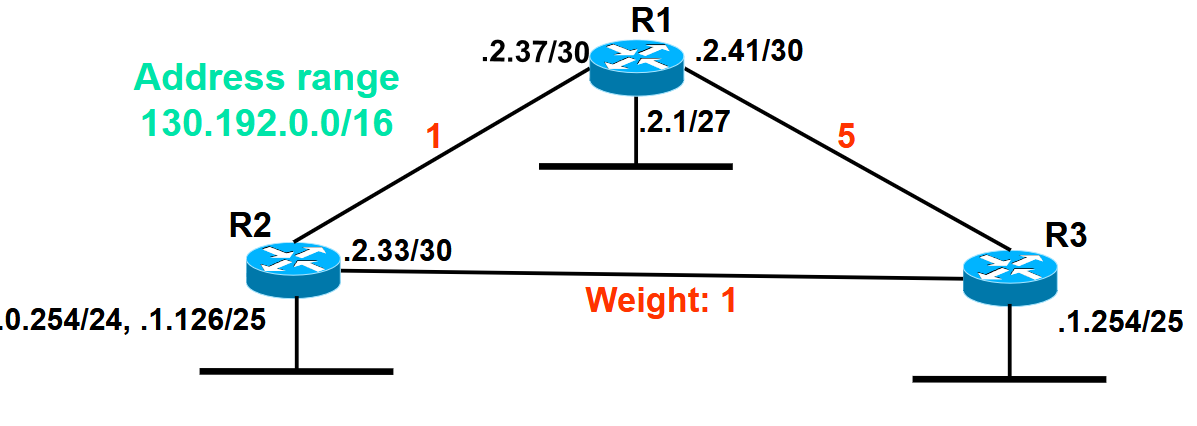
\includegraphics[width=0.6\textwidth]{capitoli/01b - IPv4 ExerciseSummary/images/topologia_aggregazione_R1}
    \caption{Topologia per il confronto tra minimizzazione indirizzi e massimizzazione dell'aggregazione.}
    \label{fig:topology_aggregation}
\end{figure}

\textbf{Scenario A (Esercizio 8): Minimizzazione degli indirizzi allocati}
Se utilizziamo l'approccio orientato solo a sprecare meno IP possibile, potremmo assegnare i blocchi in ordine di dimensione prescindendo da dove si trovino fisicamente le reti. Avremo quindi prefissi allocati dietro R2 e dietro R3 che si intersecano logicamente (ad esempio, una /25 verso R3, poi la successiva /26 verso R2, la /27 di nuovo verso R3...). 
Come risultato, la tabella di routing su R1 dovrà contenere una riga separata per ogni singola LAN. Qualsiasi tentativo di aggregazione (es. dire "tutta la /24 va a destra") fallirebbe perché creerebbe routing asimmetrico o blackhole per le reti fisicamente a sinistra, a causa del Longest Prefix Matching che dirotterebbe i pacchetti verso direzioni sbagliate. 
\textit{(Nota: Nelle slide, la tabella di routing di questo esercizio è lasciata "to be completed" proprio per evidenziare quanto diventi complessa e illeggibile a causa della frammentazione).}

\begin{figure}[H]
    \centering
    % Sostituire il segnaposto con il percorso effettivo dell'immagine
    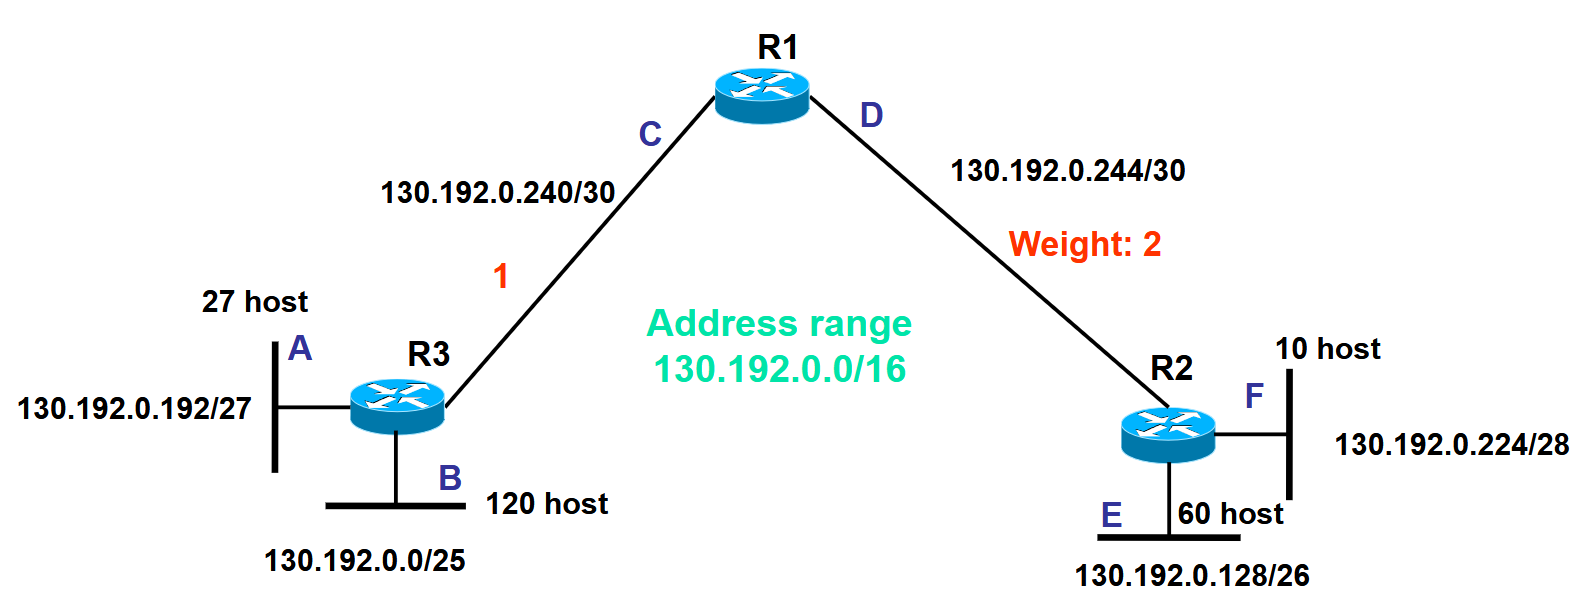
\includegraphics[width=0.85\textwidth]{capitoli/01b - IPv4 ExerciseSummary/images/routing_table_fragmented}
    \caption{Tabella di routing di R1 con allocazione frammentata (Scenario A).}
    \label{fig:routing_table_fragmented}
\end{figure}

\textbf{Scenario B (Esercizio 7): Pianificazione per massimizzare l'aggregazione}
Questo è l'approccio ideale. Invece di allocare singole LAN iterativamente da un pool globale, \textbf{si divide la rete per aree logiche topologiche}.
\begin{enumerate}
    \item \textbf{Area 1 (Dietro R3):} Comprende LAN A (32 IP) + LAN B (128 IP) + subnet intermedie = Circa 160 IP. Si alloca preventivamente e logicamente a tutta l'area una \textbf{/24} (es. \texttt{130.192.0.0/24}).
    \item \textbf{Area 2 (Dietro R2):} Comprende LAN E (64 IP) + LAN F (16 IP) = Circa 80 IP. Si alloca logicamente una \textbf{/25} (es. \texttt{130.192.1.0/25}).
\end{enumerate}
Successivamente, si creano le singole subnets per A, B, E e F \textit{solamente all'interno} dei macro-blocchi assegnati alla loro area.
In questo modo, la tabella di routing di R1 sarà estremamente sintetica e pulita:

\begin{table}[H]
    \centering
    \begin{tabular}{|c|c|c|c|}
        \hline
        \textbf{Tipo} & \textbf{Destination} & \textbf{Next-hop} & \textbf{Cost} \\
        \hline
        S & 130.192.0.0/24 & 130.192.0.161 (verso R3) & 1 \\
        \hline
        S & 130.192.1.0/25 & 130.192.0.165 (verso R2) & 2 \\
        \hline
        C & 130.192.0.160/30 & 130.192.0.162 (diretto) & 0 \\
        \hline
        C & 130.192.0.164/30 & 130.192.0.166 (diretto) & 0 \\
        \hline
    \end{tabular}
    \caption{Tabella di routing di R1 massimizzando l'aggregazione.}
    \label{tab:routing_aggregation}
\end{table}

\begin{remark}[Utilizzo della Default Route]
Nello scenario sopra esposto non vi è connessione a Internet. Sarebbe in teoria possibile utilizzare la default route (\texttt{0.0.0.0/0}) per aggregare un intero ramo. Tuttavia, se usiamo la default route per R3, non possiamo usarla per R2. È una regola forte. Inoltre, aggregazioni estreme di questo tipo diventano un problema se la topologia muta. Aggregare per macro-blocchi (es. /24 e /25) preserva la pulizia e permette futuri allacciamenti a Internet.
\end{remark}

\begin{figure}
    \centering
    % Sostituire il segnaposto con il percorso effettivo dell'immagine  
    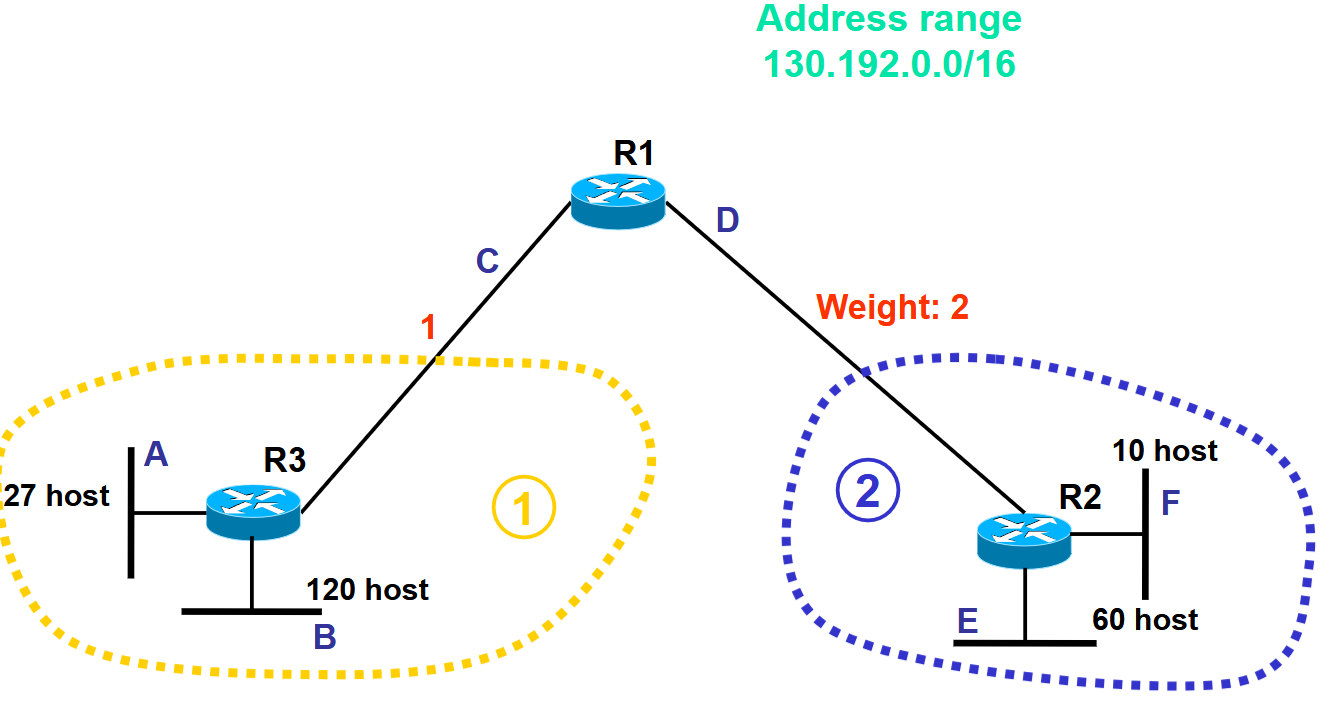
\includegraphics[width=0.6\textwidth]{capitoli/01b - IPv4 ExerciseSummary/images/routing_table_aggregated} 
    \caption{Tabella di routing di R1 con allocazione pianificata per massimizzare l'aggregazione (Scenario B).}
    \label{fig:routing_table_aggregated}
\end{figure}

\section{Analisi del Traffico di Rete e Protocolli ARP, DNS, ICMP}

Gli esercizi finali riguardano l'impatto della topologia fisica e logica sull'effettivo traffico catturato dai tool di sniffing (come Wireshark). 
Ricordiamo che in ambiente Windows, il comando \texttt{ping} invia tipicamente 4 richieste ICMP e attende 4 risposte (a differenza di Linux che invia un flusso continuo fino all'interruzione manuale).

\subsection{Ping verso un indirizzo IP nella stessa LAN}
Host A esegue il ping verso l'IP di Host B, che si trova nella medesima subnet. Le cache sono vuote. Su una LAN Ethernet a bus condiviso (Shared Bus), uno sniffer sul cavo di Host A cattura tutto il traffico.
\begin{enumerate}
    \item \textbf{ARP Request (Broadcast):} Host A chiede "Chi ha l'IP di B? Ditemi il MAC". (1 trama)
    \item \textbf{ARP Reply (Unicast):} Host B risponde inviando il proprio MAC ad A. (1 trama)
    \item \textbf{ICMP Echo Request/Reply:} 4 pacchetti di richiesta inviati da A verso il MAC di B, seguiti da 4 pacchetti di risposta. (8 trame)
\end{enumerate}
\textbf{Totale:} 10 trame. L'IP destinazione nel pacchetto è quello dell'host finale, e il MAC destinazione è quello dell'host finale.

\subsection{Ping verso un Nome a Dominio}
Se Host A pinga \texttt{www.polito.it}, interviene la risoluzione dei nomi. Non conoscendo l'IP, Host A deve contattare il \textbf{DNS} (il cui IP è noto dalle impostazioni locali).
\begin{enumerate}
    \item ARP Request e Reply per risolvere il MAC del server DNS. (2 trame)
    \item \textbf{DNS Query:} Da A al DNS per la risoluzione del nome. (1 trama)
    \item \textbf{DNS Response:} Dal DNS ad A contenente l'IP destinazione. (1 trama)
    \item Dopodiché, il processo continua come prima: ARP per scoprire il MAC del destinatario (se locale) o del Default Gateway (se remoto), seguito dai messaggi ICMP.
\end{enumerate}

\subsection{Impatto dello Switch Ethernet}
Se l'infrastruttura fisica passa da un hub (Shared Bus) a uno \textbf{Switch Ethernet}, le dinamiche di cattura di Wireshark su un singolo host cambiano drasticamente. Uno switch filtra il traffico Unicast instradandolo solo sulla porta del legittimo destinatario.
Se A pinga C (ed entrambi non sono sullo stesso cavo dello sniffer di A):
\begin{itemize}
    \item Lo sniffer su A catturerà l'ARP Request (inviata in \textbf{Broadcast}, quindi inondata su tutte le porte dallo switch).
    \item Lo sniffer su A \textbf{NON} vedrà l'ARP Reply né il traffico ICMP Unicast, a meno che il traffico non sia originato o destinato ad A stesso.
\end{itemize}

\subsection{Risoluzione DNS con Errori di Configurazione: L'Asimmetria}

Un caso didatticamente molto interessante si verifica se introduciamo un errore nella subnet mask.

% FIGURA ORIGINALE DA RECUPERARE DALLE SLIDE
% Slide di provenienza: 25
% Tipo: diagramma
% Descrizione: Host A, DNS, Router e Server Google. Host A ha subnet /24. Il DNS ha subnet /23.
% Punto di inserimento: Introduzione del problema di asimmetria
% File da inserire: topologia_asimmetria_dns

\begin{figure}[H]
    \centering
    % Sostituire il segnaposto con il percorso effettivo dell'immagine
    %\includegraphics[width=0.85\textwidth]{topologia_asimmetria_dns}
    \caption{Scenario con errata configurazione della Subnet Mask tra Host e DNS.}
    \label{fig:asymmetric_routing}
\end{figure}

\textbf{Lo Scenario:}
\begin{itemize}
    \item \textbf{Host A:} IP \texttt{130.192.16.81/24}
    \item \textbf{DNS:} IP \texttt{130.192.17.2/23}
    \item \textbf{Router:} IP \texttt{130.192.16.1/24} e \texttt{130.192.17.1/24} (due subnet logiche sulla stessa LAN fisica).
\end{itemize}
Sulla carta questo è un errore in quanto un admin voleva digitare /24 sul DNS ma ha digitato /23. Cosa comporta a livello di cattura pacchetti?

\textbf{L'Asimmetria:}
A causa della discrepanza delle subnet mask, le macchine non concordano sulla reciproca appartenenza alla stessa rete.
\begin{enumerate}
    \item \textbf{A $\rightarrow$ DNS:} Per Host A (\texttt{/24}), il DNS che inizia con \texttt{17} risiede in una rete remota. Di conseguenza, A invierà il pacchetto al Router. L'ARP Request di A cercherà il MAC del \textbf{Router}. La query DNS, a livello MAC, è indirizzata al Router, ma a livello IP è indirizzata al DNS. Il Router, ricevendo la query, la instraderà (inviando a sua volta un ARP per il DNS) verso il DNS.
    \item \textbf{DNS $\rightarrow$ A:} Per il DNS (\texttt{/23}), l'indirizzo di A (\texttt{16.81}) ricade all'interno della propria subnet locale (infatti \texttt{130.192.16.0/23} ingloba sia la .16 che la .17). Il DNS quindi non interpellerà il Router. Invierà un'ARP Request in broadcast per cercare l'IP di A. Una volta ottenuto, invierà la \textbf{DNS Reply direttamente al MAC di Host A}.
\end{enumerate}

Questo genera un flusso asimmetrico: il pacchetto d'andata passa dal router, il pacchetto di ritorno avviene direttamente a livello MAC.
Paradossalmente, in molti sistemi \textbf{questa configurazione errata continua a funzionare}. Livello 2 e Livello 3 (l'ARP non fa menzione della subnet) gestiscono l'invio fisico; fintanto che i protocolli di sicurezza dei SO non bloccano i pacchetti asimmetrici, l'utente potrebbe non accorgersi mai del problema se non ispezionando l'indirizzamento sorgente o i tempi di risposta tramite un'analisi con Wireshark.




